\documentclass[11pt, oneside]{article}   	% use "amsart" instead of "article" for AMSLaTeX format
\usepackage[margin=1in]{geometry}                		% See geometry.pdf to learn the layout options. There are lots.
\geometry{letterpaper}                   		% ... or a4paper or a5paper or ... 
%\geometry{landscape}                		% Activate for for rotated page geometry
\usepackage[parfill]{parskip}    		% Activate to begin paragraphs with an empty line rather than an indent
\usepackage{graphicx}				% Use pdf, png, jpg, or eps� with pdflatex; use eps in DVI mode
\usepackage{lipsum}
\usepackage{hyperref}
\usepackage{cleveref}				% TeX will automatically convert eps --> pdf in pdflatex		
\usepackage{amssymb}
\usepackage{sectsty}

\usepackage{titlesec}
\setcounter{secnumdepth}{4}
\titleformat{\paragraph}
{\normalfont\normalsize\bfseries}{\theparagraph}{1em}{}
\titlespacing*{\paragraph}
{0pt}{3.25ex plus 1ex minus .2ex}{1.5ex plus .2ex}

\sectionfont{\fontsize{12}{15}\selectfont}

\newcommand{\subsubsubsection}{\paragraph}
\newcommand{\la}{\emph{Later }}
\newcommand{\now}{\emph{Now }}


\title{Parallel Path Finding}
\author{Stephan Boettcher}
%\date{}							% Activate to display a given date or no date

\begin{document}

\maketitle
\begin{figure} [!h]
  \centering
    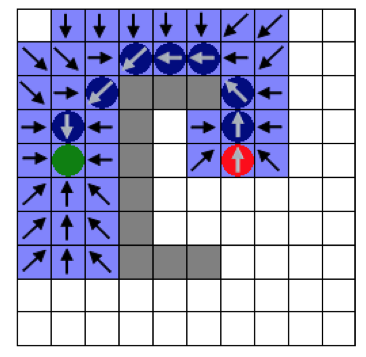
\includegraphics[width=0.5\textwidth]{moo.png}
\end{figure}
\newpage

\tableofcontents
\newpage
\section{Introduction}
Unmanned Aerial Vehicles have been a part of our society and military for over 150 years. Initially used in military settings, these vehicles have increasingly been permeating civilian society. As computational power increases as the cost for high-speed chips decreases, the overall cost to develop and own a small UAV has dropped drastically. Many of these small civilian UAVs currently have small payload capacities and limited range due to battery power restraints. However, as battery technology continues to develop, these limitations will have less of an impact on drone range, speed and carrying capacity.  As the cost to develop and operate these UAVs decreases, a number of corporations have begun to investigate integrating these systems into their supply and delivery chains. 

\section{Motivation}
Amazon Prime Air\cite{amazon} was announced December 2013 as a way to deliver packages within 30 minutes of ordering. In August 2014, Google\cite{google} announced its own drone delivery project. Each of these projects place restrictions on which customers are able to utilize this service, usually based on a geographic radius from a supply warehouse. To achieve optimal efficiency, these drones will need to fly from the warehouse to their delivery location following an optimal path. Ideally, these corporations would be able to generate a static maps of the areas surrounding their warehouses and pre-calculate path segments to generate these paths quickly and efficiently. Unfortunately, this is not always possible. In a dense, urban environment such as Los Angeles, airspace restrictions are fluid and subject to change over the course of a day. 

Restrictions of airspace can come from many different sources. Should a fatality occur on one of the many overcrowded highways occur, or a shooting in a residential neighborhood occur, the local police or highway patrol will restrict the airspace surrounding the incident. The FAA also places temporary no-fly-zones surrounding large events such as sporting events or major political events and permanent airspace restrictions surrounding airports. As FAA guidance surrounding the use of UAVs develops, further restrictions may be placed upon their use and paths. All of these factors create a dynamically changing environment through which the UAV will need to traverse. 

Many path generation algorithms have been proposed and perfected since the 1960s, most notably of these being the A* algorithm. The A* algorithm, is an optimal path-finding algorithm that has been adapted by many game platforms. This algorithm is guaranteed to find the optimal path, should one exist. The A* algorithm achieves this because it maintains an ordered list of tested nodes, and is able to choose the lowest cost path from this node list. Unfortunately, keeping this list ordered makes parallelizing the algorithm difficult. Other search methods include the fringe search algorithm. The Fringe Search (FS) method does not require the use of an ordered list of nodes to determine a path, but as a result cannot guarantee optimality. Thus, the FS algorithm trades optimality for speed. This project explored this speed vs optimality trade off as well as explored the best way to quickly generate a large volume of optimized delivery paths. 

\section{Literature Survey}
Path finding algorithms were created early in  field of computer science, first with Dijkstra's algorithm (1959), and later with the creation of the A* algorithm (1968). The A* algorithm uses  a distance-plus-cost heuristic function to determine the order which graph nodes are visited while searching for the optimal path, if it exists, from point A to point B. To do this, the A* algorithm traverses a graph, following a path of lowest know heuristic cost while keeping a sorted list of alternative path segments\cite{Dong}. The result is the least-cost path from the initial node to the target node is chosen out of the sorted list as the shortest path, thereby guaranteeing an optimal path between the nodes. This method of path-finding has popular in gaming, logistics, navigation, CAD systems\cite{Szabo}, and mission planning since its creation. As hardware systems continue to improve, the use of A* path finding algorithms in games, such as Massive Multi-Player On-line Role Playing Games (MMORPG), has increased\cite{Botea}\cite{Inam}\cite{Gedge}\cite{Nohra}\cite{McNally}\cite{Szabo}. However, as the number of Artificial Intelligence (AI) players increase, the computational load of creating and maintaining paths for these characters over complex terrain has increased drastically. In its current state, the A* algorithm does not scale well to multiple processors of a distributed architecture\cite{Accaputo}. Many gaming platforms currently dedicated threads and processor cores to just calculate A* paths\cite{Nohra} as a viable method of parallelizing. Attempts have been made to directly parallelized the A* algorithm \cite{Accaputo} but ended poorly. Other researchers have focused on other path finding algorithms based on A*\cite{Brand}.

\subsection{Parallelization of the A* Algorithm}
The goal of parallelizing the A* algorithm is to achieve the greatest amount of speedup to minimize the algorithm runtime. A number of different modifications to the Dijkstra algorithm (of which, A* is a subset) to achieve this speedup. Because the A* algorithm needs to maintain a sorted open list, and thus may need to correct said list as nodes are opened and closed, achieving a good scale up of the algorithm is difficult. By using the Hierarchical A* Algorithm and using OpenMP, speedups can be achieved but are challenging due load balancing issues\cite{Miller}. An easy way to involve two cores in the A* search is to begin the search at both end nodes in a Parallel Bidirectional Search(PBS)\cite{Brand}. While the PBS algorithm employs the same A* algorithm, as the serial version, it is possible that the path in the area around the intersection is not strictly optimal, as not all nodes around the intersection may be fully flooded.

Another method seen in the literature to achieve speedups is the use of pre-stored paths. If the A* algorithm has been run on an area, so long as no changes have occurred on the path length (e.g. dynamic barriers), there is no need to recompute the length. Another implementation of the A* uses 'multiple threads per agent\cite{Inam} to work on a small subset of the path as a group. A master thread maintains control of the execution and executes the choice of 'current node'. Thread synchronization is required for this version, resulting in a number of threads sitting idle while the master thread executes the serial code. Another way to achieve speedups of the A* algorithm is to 'find the A* oath hierarchically\cite{Botea}.  This 'multiple thread per agent' algorithm must have an modified termination condition from that of the A* method. The program must not terminate immediately upon finding a path or else it may report a suboptimal solution, instead it is suggested that a global flag should be set to true indicating that  a path has been found\cite{Cohen}.

\subsection{Other Parallel Path Finding Algorithms}  
A path finding algorithm's goal is to find the optimal path from point A to point B. However, if the constraint of strict optimality can be relaxed, large gains in performance can be realized. All of the following algorithms described are based off of the A* search or are in the same family as the A* search. 

A Fringe Search (FS) is based off of an A* algorithm, but instead of maintaining a sorted list of open and closed nodes, it uses a \now list and a \la list. The \now and \la lists do not need to be sorted and thus cut out a costly portion of the A* algorithm. Because the nodes are not sorted, nor does the FS need to maintain any kind of sorted array, the path that is ultimately generated is no longer guaranteed to be optimal\cite{Brand}. However, studies have shown that the FS algorithm is usually within a few percentage points of being optimal. The FS algorithm also lends itself to being scaled up and parallelized more readily than the A* algorithm. The first way is with the Distributed Fringe Search (DFS). The DFS takes the \now nodes in the FS algorithm and disburses them over multiple cores. Each core then computes the smallest f(n) value found locally and pass that value to a master core to do comparisons. A drawback of the DFS algorithm is that the it is no longer possible to keep track of the parent-child relation of nodes during flooding. This information is needed to reconstruct the resulting path. As a result, a shared buffer must be used to signal to each other who is the owner. Care must be taken to avoid race conditions in the shared buffer, which may cause a drop in performance\cite{Brand}. 

Another way to utilize the cores available in a CPU or GPU is to have each core find a small segment of the overall path. This can be done if a high-level graph is first generated to create potential waypoints on the route. Once the high-level graph has been created, a Parallel Hierarchic Search (PHS) can then be implemented. A PHS creates a path through the high-level graph and then find sub paths connecting the anchor nodes. A "beautification" step is then applied to create way-points half way between the path segment nodes to help find "shortcuts" between the high-level anchor  waypoint nodes. The path segments are then calculated over multiple cores. The PHS suffers from a 'critical section' in the code that is required to allow safe access to selecting path segments and returning path segment solutions. This can greatly impact the performance of the algorithm. The Parallel Ripple Search (PRS) attempts to remedy this. The PRS uses the same high-level graph as the PHS but now finds path segments doing a normal A*-like search to the nearest neighbors. As each core foods the graph, the 'ripples' will eventually overlap and hopefully shortcuts can be uncovered. The PRS is also good at dealing with dynamic obstacles in the path\cite{Brand}. 

\section{Methodology}
This project attempted to explore the trade space between generating one path as fast as possible vs generating many paths at once. A single path can be generated extremely quickly using an algorithm similar to the Parallel Ripple Search or Fringe Search, but at the cost of hogging resources. Conversely, it is possible to spawn off one path per thread and batch process the paths using a slower serial algorithm. To find how to generate the most paths possible in a given time, and thus get the most packages out the door, this trade space must be explored. 

Both the A* algorithm and the Fringe Search algorithm were parallelized in some fashion. The A* algorithm by its very nature lends itself to being a serial algorithm, with very little parallel slack, while the Fringe Search algorithm can be parallelized more easily. 

\subsection{Maps}
A baseline map set were used to benchmark the effective calculation speed of the different parallel methods. These maps differ in size and complexity, to mimic different flight path lengths. A large map mimics a UAV traveling far from the base warehouse location, and a small map mimics a much shorter flight path. In the end, 6 maps were created for use in this benchmarking suite. To force the algorithms to traverse a decent portion of the map, a minimum path length was determined by each map using the following formula:
$$
L_{path}= \sqrt{(X_{start}-X{end})^2 +(Y_{start}-Y_{end})^2} \ge \frac{Map\_Width}{2} 
$$
Where X and Y are the pixel locations on the map and $X_{start},Y_{start}$ always are 0. Thus, the algorithms must traverse a quarter circle area with a radius equal to one of the map lengths, before it can have a valid endpoint. This was done to eliminate extremely quick run times caused by short paths. 
\begin{figure}[htbp]
\begin{center}
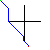
\includegraphics[width=40mm]{Run_0.png}
\caption{Small Cross Map. 50x50 pixel, with a start point of (0,0)}
\label{Small}
\end{center}
\end{figure}
%\vspace{3mm}
The first and smallest map is a simple cross. This map is the most basic map used in the benchmarking set and simulates close by deliveries in an area with minimal restrictions. Other more complex 50x50 local area maps can be found in Appendix A. These other maps simulate more dense and restrictive local area deliveries.


\vspace{3mm}
\begin{figure}[htbp]
\begin{center}
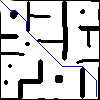
\includegraphics[width=60mm]{Run_1.png}
\caption{Medium  Map. 100x100 pixel, with a start point of (0,0)}
\label{Med}
\end{center}
\end{figure}

The medium map found in Figure \ref{Med} contains a more complex map that would simulate a medium distance flight path for the UAV. As can be seen in Figure \ref{Med}, there are a number of obstacles, no-fly-zones and general impedances to the UAV flight path. 



The Large Geometric Map found in Figure \ref{Geom} is a more unusual map. While initially it may seem to bear little relevance to a UAV path, it actually simulates two important phenomenon. The first is this map contains an area that cannot be reached. This is used to test the algorithm logic for unreachable paths, which due to airspace restrictions may pop up. The second is this simulates a potential entrance into restricted airspace. When entering such airspace it is not usual to have to enter from a certain vector and geographic location. An aircraft may also be forced to circle the intended location prior to final descent while the airspace clears or to circle areas of airspace that will not become available. 

\vspace{3mm}
\begin{figure}[htbp]
\begin{center}

\includegraphics[width=100mm]{Run_2.png}
\caption{Large Geometric Map. 1000x1000 pixel, with a start point of (0,0)}
\label{Geom}
\end{center}
\end{figure}

The Large Area of Regard map in Figure \ref{AOR} simulates an extremely restricted airspace with multiple Class B,C and D airspaces. Class B airspaces are generally large areas placed around large important airports, such as LAX in Los Angeles. Class C  airspace is placed around smaller, less important airports such as the Burbank, Orange County and Long Beach airports in Los Angeles. Class C airspaces are smaller than Class B, but would still be restricted to UAV flights without prior authorization and coordination. Class D airspaces are generally smaller than Class C and is generally placed around small municipal airports. Other small restricted areas on this map simulate other restricted airspaces. The actual Los Angeles Visual Flight Reference (VFR) map provided by the FAA is found in Figure \ref{LAX} in appendix A.

\vspace{3mm}
\begin{figure}[htbp]
\begin{center}
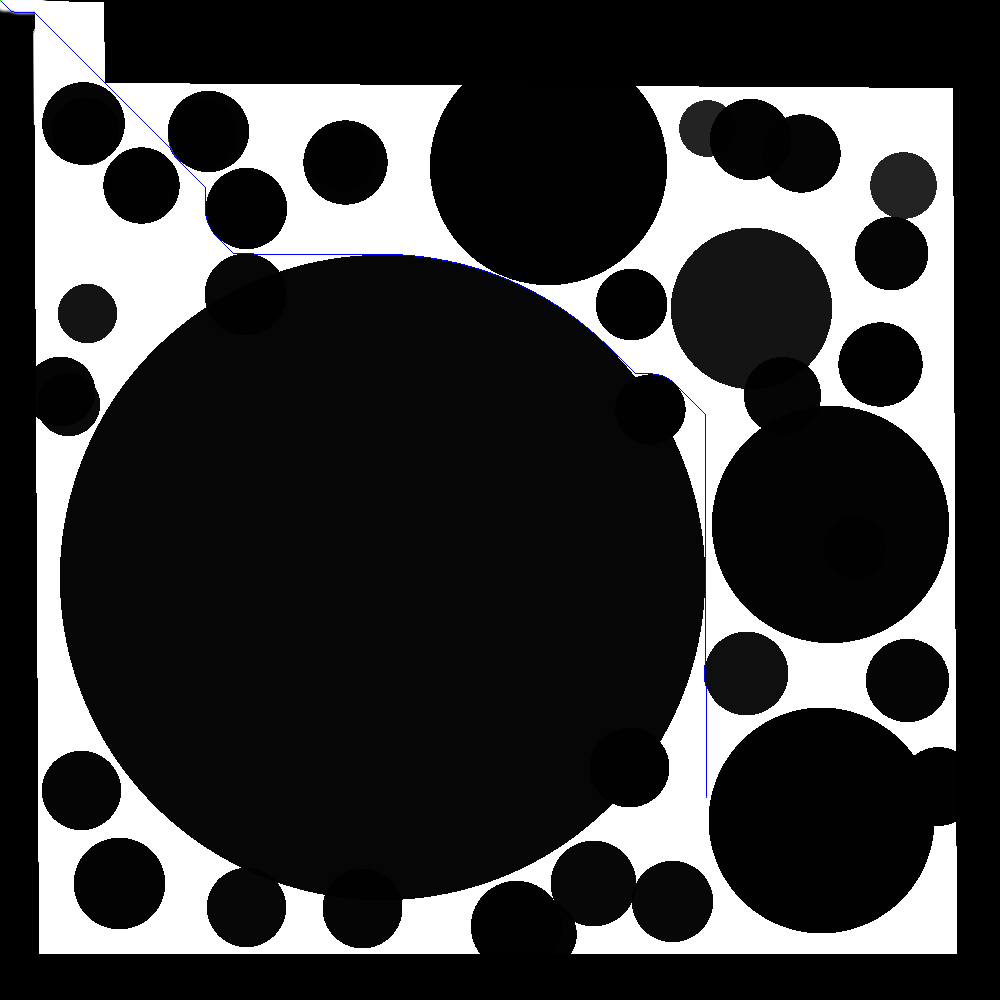
\includegraphics[width=100mm]{Run_3.png}
\caption{Large Area of Regard Map. 1000x1000 pixel, with a start point of (0,0)}
\label{AOR}
\end{center}
\end{figure}



\subsection{A*}
The A* algorithm was first custom coded to better grasp the intricacies involved in pathfinding algorithms, but later a library form of the algorithm was used. The final analysis was performed on the library code, rather than the custom code for the sake of consistency.  A baseline measurement was taken with the serial A* code for use in later comparison. After this was complete, the A* code was parallelized in two ways: Batch mode and Batch parallel mode. Each of these two modes were parallelized using Cilk and OpenMP, to compare the relative speed between the two methods. Finally, the A* code was run in a distributed fashion using OpenMPI.

\subsubsection{Batch}
The code was run in a batch processing mode first to see the effects of running the serial code on multiple threads. This was accomplished by using either a {\bf cilk\_for} or an {\bf\#pragma parallel} and {\bf\#pragma for} command in the driver code. While this does not actually parallelize the A* algorithm, this is the current method used by many gaming platforms to calculate paths. 

\subsubsection{Batch Parallel}
In the Batch Parallel mode, the A* algorithm is parallelized as much as possible. Unfortunately, this algorithm does not lend itself to being parallelized. When the algorithm is executing, it begins the node with the lowest cost from a sorted list. The algorithm then begins to open the nodes surrounding this low cost base node to find the next step. All of these newly open nodes are then put into the sorted queue to be explored, and the base node is closed. The algorithm then repeats this process until a path to the final node is found. Because of the way this algorithm maintains a sorted list of open nodes and the large potential for race conditions in exploring nodes, parallelization must be preformed carefully. The best way to parallelize the algorithm is to use multiple threads to explore the nodes surrounding the base node. This allows the code to speed up without the hazard of race conditions. This was performed with Cilk and OpenMP.

\subsubsection{MPI}
With MPI, the code was run in a distributed, batch  and batch parallel manner. This simulated the method a large data center would be expected to employ to crunch through the data. In this setup, a central processor controls the execution process via communication with the other nodes. The central node sends basic parameters such as start/stop points and which map to execute, to each of the computational nodes. Each node is then responsible for loading up the map and finding the best path. Once a path has been found, the final output parameters, such as path execution time, path length, and if it was a success, are transmitted back to the main node. To minimize communication time between the central processor and the nodes, the actual path is not transmitted. Each node is held accountable for outputting the final path. 


The two factors heavily investigated with all of the MPI code were the size and type of messages passed to each node and the setup of the scheduler. The size, type and quantity of messages sent by the central control node is known to have an impact on the overall performance of the code. As such, the effect of this factor was explored. The initial message structure consisted of a large message containing all of the data necessary for a run. Subsequent message iterations pared down this message to a smaller, sparser message that contained only the bare minimum information necessary to run. This was done to cut down on the bandwidth consumed by each message. The second effect investigated was the setup of the scheduler. Based on the message latency, it was posited that some of the small maps would have faster runtimes than the cost to send the message. If this proved correct, it would be faster to run some, if not all, of the smaller maps on the local processor. As this was investigated, the order in which the local maps vs sending messages was also investigated. 

\subsection{Fringe Search}
The Fringe Search (FS) method was used as a more easily parallelized, semi-optimal, path-finding algorithm. The FS algorithm uses two node lists that are unsorted to keep track of which nodes have been explored and which nodes are yet to be explored. This method effectively maintains an exploration front line, where behind the front line all nodes have been explored and all nodes outside of the front line need to be explored. The FS method was run in a Batch and Batch parallel mode to compare the effective speed of calculation. 

\section{Results}
%%%%%%% RE READ THIS SECTION!!!!!!!!
Overall, the A* algorithm proved difficult to speed up. The largest gains were observed with the OpenMp code running in batch parallel mode and with all available cores working. This was surprising, as the MPI Distributed Batch Parallel code was expected to run the fastest. However, some restrictions in the MPI method led to inefficiencies in the scheduling of cores. Even with a custom, refined scheduler, the MPI code was unable to achieve the speeds seen on a single jinx cluster running in a local batch parallel mode. To achieve the speedups seen in the sections below, the runs had to be analyzed and preprocessed. The Fringe Search method, with the restrictions placed upon it by the nature of UAVs, proved to be minimally effective. The loss of path optimality, even if only ~2-10\%, results in a longer flight time than path calculation runtime gained, and thus would result in the UAV taking longer to deliver a package. This surprising result is detailed further in the Fringe Search section.

\subsection{A*}
The A* algorithm is an extremely efficient serial algorithm used to calculate the optimal path from point A to point B. In this project, the algorithm was run in a parallel, batch parallel, and distributed mode. 

\subsubsection{Serial}
The serial code was run as an initial benchmark for the parallel algorithms. On average, it took the serial code 150 seconds to execute 1000 map iterations, with all 6 maps utilized. Figure \ref{SM} outlines the average runtime per map, as well as the average path length for these maps.

\begin{figure}[htbp]
\begin{center}
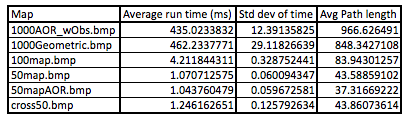
\includegraphics[width=90mm]{SerialMap.png}
\caption{Average Map runtimes and path lengths }
\label{SM}
\end{center}
\end{figure}

As can be seen by the standard deviation column, there was minimal variance in how long it took the code to execute. This is expected as only system loading and other processes will effect the repeatability of the run times. The small standard deviation shows that these system level random variables have minimal impact. 

\subsubsection{Batch}
The first parallelization attempt was the na\"ive and simplistic method of spawning a number of threads to run the serialized code in parallel. This was done in both Cilk and OpenMP to compare their relative efficiency in thread spawning, as well as to determine any performance differences. The final results showed that in batch mode, OpenMP and Cilk were equivalent  at the batch processing method, as seen in Figure \ref{CvMP}. The minor difference in runtime may be attributed to system loading issues and other non-deterministic effects. 

\begin{figure}[htbp]
\begin{center}
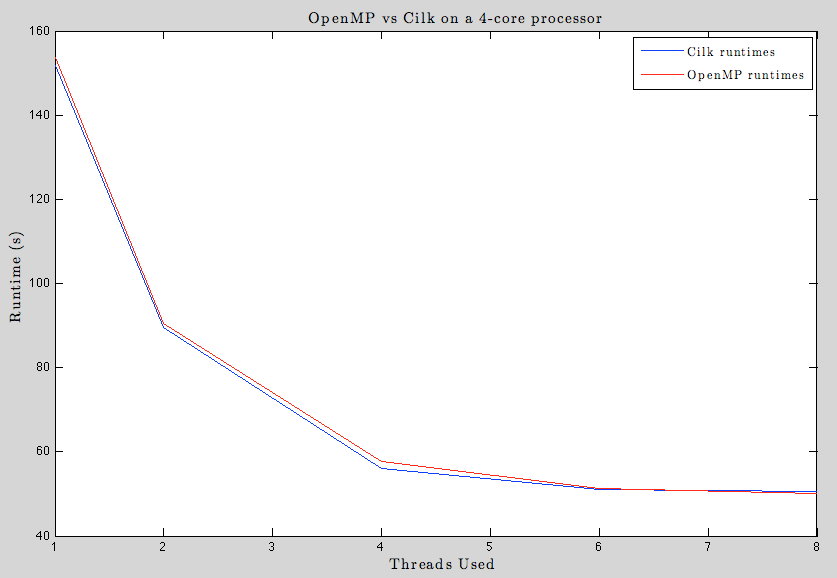
\includegraphics[width=90mm]{CvMP.png}
\caption{Runtime of 1000 iterations in Batch mode on Cilk and OpenMP}
\label{CvMP}
\end{center}
\end{figure}

With the code running in Batch mode on a 4-core processor, speedups of approximately 3x were seen. This was below the expected 4x speedup expected but further investigation into the system showed that only 3 of the processors were actually fully dedicated to the task. Thus the slightly above 3x improvement falls in line with expectations. 

Ultimately, OpenMP was chosen for implementation on the Jinx clusters, mostly due to software support issues. The OpenMP code was easier to manage and compile with the C++11 standard used by the A* code than Cilk. 

Finally, this code was run on 8 Jinx nodes using the MPI standard. In this setup, one thread was the control thread and spun messages off to a number of other threads located on the other nodes. The MPI standard allows the user to determine how many processes are used to run the code. This feature was used to control the amount of parallelism used by the code. Initially, the code was only run with 2 processes. This mimics the serial code as only one process is actually performing the calculations. This was done to gauge the communication time that must be overcome by the parallelism to make MPI worthwhile. As seen in Figure \ref{Stime}, there is a very real communications penalty with MPI, resulting in an approximately 50\% increase in runtime. For 1000 runs, this puts the communication cost at 79 milliseconds per run. 

\begin{figure}[htbp]
\begin{center}
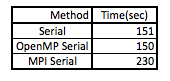
\includegraphics[width=45mm]{Stimes.png}
\caption{Comparison of Serial Runtimes}
\label{Stime}
\end{center}
\end{figure}

The 79 millisecond communications cost greatly dwarfs $\frac{4}{6}$ of the average runtime costs as seen in Figure \ref{SM}. However, for the first attempt using MPI, all of the maps were still sent with MPI messages. This was done in the hopes that with a large number of processes running, the communications cost would be hidden. As seen in Figure \ref{MPIr}, with multiple processes, the communications cost of MPI can indeed be greatly hidden. The MPI parallelization method was able to achieve a final runtime of 32 seconds when run with 32 processes.  

\begin{figure}[h!]
\begin{center}
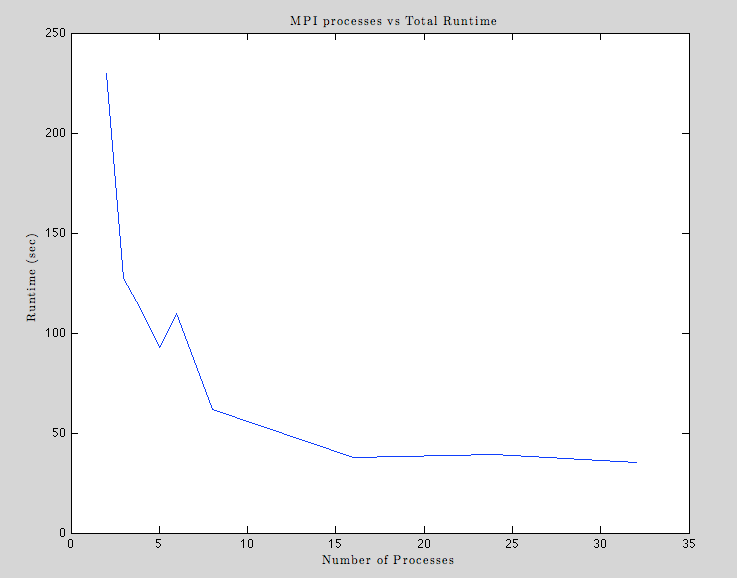
\includegraphics[width=90mm]{MPIbrun.png}
\caption{MPI Runtimes}
\label{MPIr}
\end{center}
\end{figure}

Further attempts to optimize the MPI scheduling process were attempted. This was done by having the base processor run all of the smaller map cases, thereby removing the communication cost. This updated scheduling process proved  to have minimal runtime gains. Due to a busy scheduler process, it was not any more efficient to process the smallest maps on the local core than incur the communications costs, as seen in Figure \ref{MPIr2}. 



Unfortunately, the MPI code was unable to fully hide the communications cost incurred during the message passing phase. Load balancing and more active communication between the scheduler and the various nodes may be a way to decrease the final runtime. I was noticed during the final analysis period that some of the MPI processes were finishing before others and exiting out of the program. Future research into efficient MPI scheduling may result in further gains.
\begin{figure}[h!]
\begin{center}
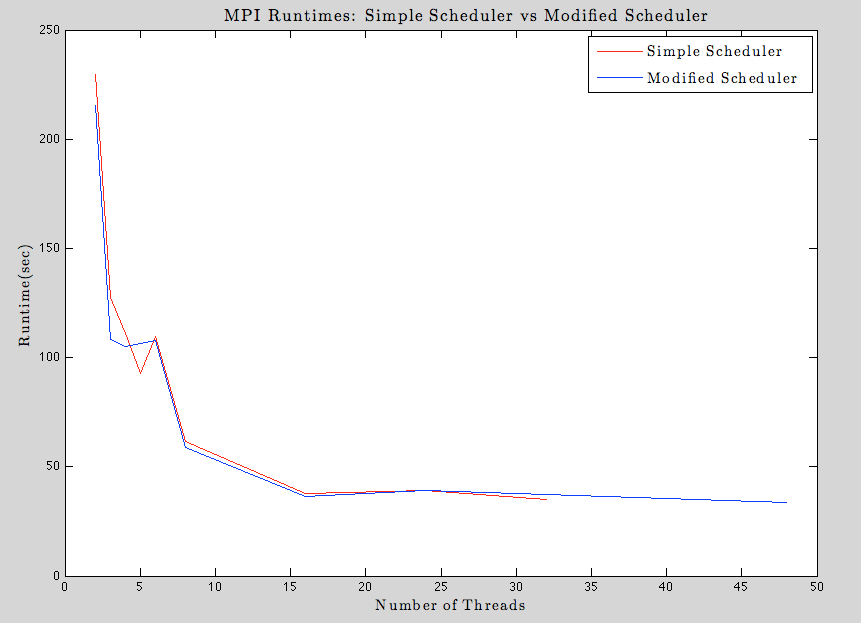
\includegraphics[width=90mm]{MPIbrun2.png}
\caption{MPI Runtimes with the modified scheduler vs initial scheduler.}
\label{MPIr2}
\end{center}
\end{figure}

\subsubsection{Batch Parallel}
The second and more in-depth attempt at parallelization did not just look at spinning off the processes in a batch serial manner. The Batch Parallel version attempted to actually parallelize the A* method. As stated in the Methodology section above, the best way to parallelize the A* method while maintaining optimality and avoiding race conditions is use multiple threads per agent. This method uses multiple threads to explore potential new nodes surrounding a base node. For example, the starting node is surrounded by 8 possible new nodes and as a result, 8 possible directions to move. In this case, up to 7 additional threads could be used to explore the surrounding nodes, calculate their relative weight, and add them to the queue. The queue is then sorted by one thread, to maintain an ordered set. While this parallelization method is not as fast as a sub-optimal path generation program, it does result in speedups. 
\begin{figure}[h!]
\begin{center}
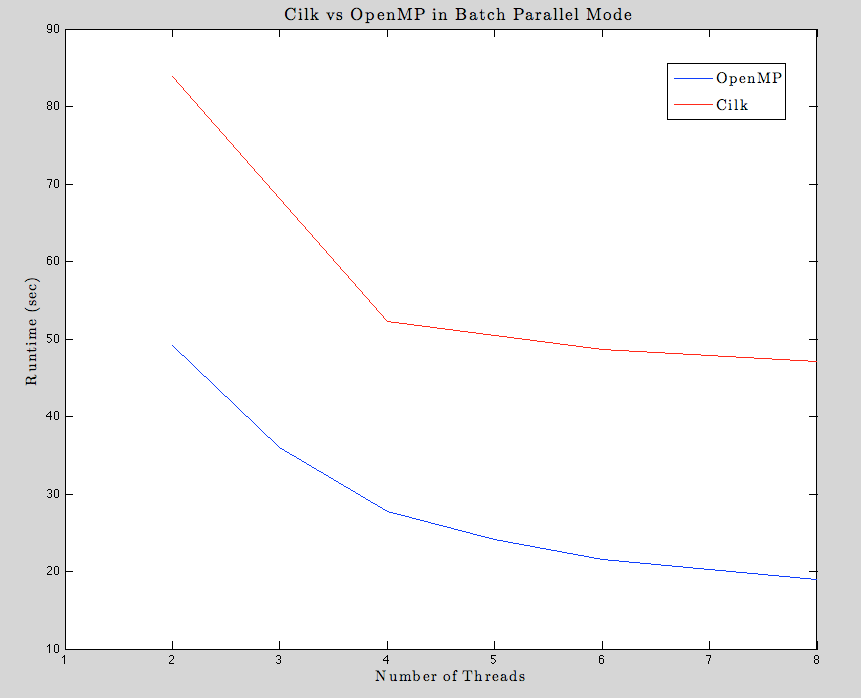
\includegraphics[width=90mm]{OMPvCilk_bp.png}
\caption{Runtimes of OpenMP and Cilk in Batch Parallel mode}
\label{MPvC}
\end{center}
\end{figure}

The Batch Parallel method was implemented first in Cilk and OpenMP. The additional parallelization achieved moderate gains with in the Cilk implementation, but large gains in the OpenMP implementation. The disparity between the two methods comes from the way that the number of Cilk threads is set, as well as the number of processors used. Cilk uses an environmental variable to set the number of workers. This is set at the start of the implementation to control the number of batches created. However, since each thread is now assigned to a process, there is little spare processing power. In the OpenMP implementation, the number of batches can be set at the parallel section, and later in the code, the number of workers can be opened up so that any free threads can be utilized. The OpenMP code was also run on the Jinx cluster, whereas the Cilk code was run on a personal computer equipped with a 4-core i7 processor. This may also account for some of the differences in speed. Figure \ref{MPvC} shows the performance of the Cilk code vs the OpenMP code.




Once the Batch Parallel modes were established, the OpenMP version was integrated with MPI. This resulted in a Distributed Batch Parallel configuration. This configuration used the same best-case scheduler discussed in the Batch mode for MPI. The OpenMP Distributed Batch Parallel configuration failed to live up to expectations. The same issue seen in the MPI Batch code was seen in the Batch Parallel code. The parallelization of the A* algorithm had minimal impact, most likely because all of the threads were assigned to a set of maps. Only once a thread had finished executing its map set would it be free to help other threads on the local processor execute their map sets. Figure \ref{MPbp} shows the final speedup of the MPI code. As can be seen in Figure \ref{MPbp}, the extra speed from the OpenMP code running in Batch Parallel was still unable to overcome the communication costs. Future project may further explore ways to optimize the message passing setup to achieve better speedups.

\begin{figure}[h!]
\begin{center}
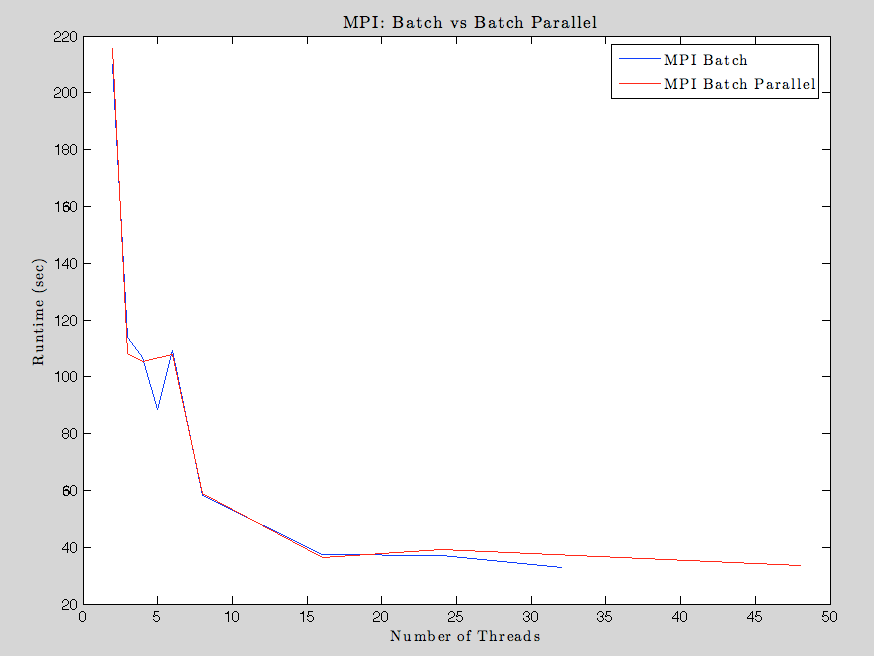
\includegraphics[width=90mm]{MPI_bp.png}
\caption{Runtimes of MPI in Batch Parallel mode}
\label{MPbp}
\end{center}
\end{figure}

Overall, the A* algorithm was sped up 12x with the OpenMp code running in Batch Parallel mode. While this is less then hoped for, multiple methods and languages were used to attempt a mass speedup. Figure \ref{Alldata} shows the final runtimes of all the methods attempted. As can be seen from the figure, the OpenMP code running in Batch Parallel mode is able to achieve the greatest speedup with the least amount of resources used. The OpenMp Batch Parallel code was able to achieve a peak runtime of 18 seconds when running on all 6 cores on the Jinx cluster. 


\begin{figure}[h!]
\begin{center}
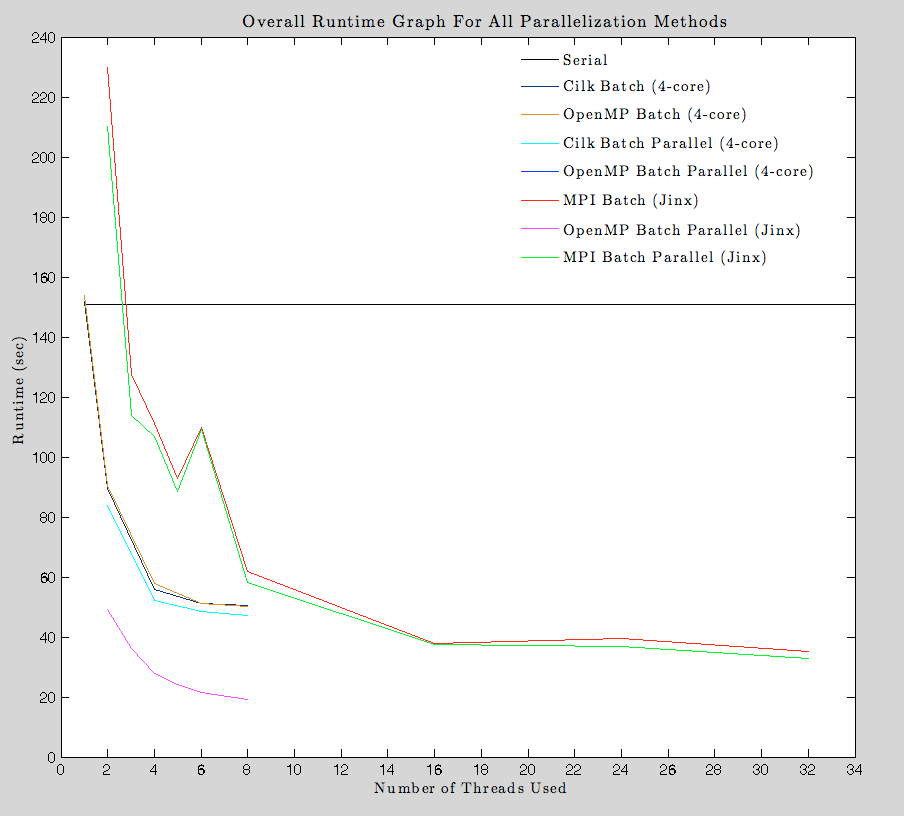
\includegraphics[width=140mm]{Alldata.png}
\caption{Total speedup graph of all the methods implemented}
\label{Alldata}
\end{center}
\end{figure}

\subsection{Fringe Search}
The Fringe Search(FS) method was originally considered as an alternative to the A* as it would be able to be parallelized more readily. However, a starting comparison with the serial A* and serial FS codes revealed that FS ran ~50\% slower than the A* code. Regardless, this code was used to create a batch and batch parallel mode. In a batch parallel configuration, the FS code ran ~10\% faster than the A* code, but at the cost of optimality. From the literature survey, the average loss of optimality was 2-10\%. Given the maximum real world, round-trip distance a drone can travel is ~ 1 hour from the base station, according to Amazon. Thus, a drone can fly 30 minutes, accounting for flying under loaded conditions, weather and other adverse conditions. It was realized that a 2-4\% path optimality loss would result in a loss of 1-6 minutes of flight time, depending on path length. While this seems like a minimal loss, over 1000 runs this adds up to more than 1000 minutes of loss productivity, just for using the FS method. While parallelizing this algorithm was a good exercise in programming, the FS method failed to provide sufficient gains to be considered a viable solution for UAV path generation. 


\section{Conclusion}

Overall, the A* method is a fairly efficient path finding algorithm. While it is somewhat difficult to drastically parallelize this code while still maintaining optimality, sufficient parallelization options were available to achieve large speed ups. While utilizing the OpenMP code in Batch mode, a linear speedup was achieved. The effects of message size, quantity and type were investigated, as were the effects of combining multiple parallelization paradigms. Ultimately, the economic limits and physical constraints surrounding the use of UAVs as a package delivery system dictated the largest constraints on the project. Had the path generation runtimes been longer than the added flight time of a drone on a suboptimal path, other path-finding algorithms could have been utilized and parallelized. Further studies could be directed to determine the optimal message structure and scheduler setup to get further parallelization gains. However, the time-constrained nature of the semester restricts this investigation currently.  Regardless, a linear speedup of the runtimes was achieved under these restrained conditions and a large number of complex paths were able to be calculated in a short timeframe.


\pagebreak
\begin{thebibliography}{99} 
\addcontentsline{toc}{section}{References} 

\bibitem{Accaputo}  Accaputo, Giuseppe, and Pascal Iselin. "Parallel A* Pathfinding Algorithm." SPCL - Scalable Parallel Computing Lab. ETH Z�rich, 16 Dec. 2013. Web. 1 Oct. 2014. 

\bibitem{Allen} Allen, T. L. (2011). Time-optimal active decision making. Thesis. Retrieved 1 Oct. 2014. 

\bibitem{amazon} "Amazon Prime Air." Amazon Prime Air. Amazon, n.d. Web. 24 Nov. 2014.

\bibitem{Brand} Brand, S., \& Bidarra, R. (2012). Multi-core scalable and efficient pathfinding with parallel ripple search. Computer Animation and Virtual Worlds, 23(2), 73-85. doi:10.1002/cav.1427 13 Oct. 2014. 

\bibitem{Botea} Botea, A., M�ller, M., \& Schaeffer, J. (2004). Near optimal hierarchical path-finding. Journal of Game Development, 1(1), 7-28. Retrieved 13 Oct 2014

\bibitem{Cohen} Cohen, D., \& Dallas, M. (2010). Implementation of parallel path finding in a shared memory architecture. Department of Computer Science Rensselaer Polytechnic Institute: Troy, NY. Retrieved 1 Oct. 2014. 

\bibitem{Dong} Dong, G., Fu, X., \& Xue, H. (n.d.). An improved A* algorithm and implementation for pathfinding in symmetrical circumstances. Retrieved 1 Oct. 2014. 

\bibitem {Gedge} Gedge, J. (n.d.). Parallel search for map-based pathfinding. Retrieved 1 Oct. 2014. 

\bibitem{google} Madrigal, Alexis C. "Inside Google's Secret Drone-Delivery Program." The Atlantic. Atlantic Media Company, 28 Aug. 2014. Web. 25 Nov. 2014.

\bibitem{Inam} Inam, R. (2010). A* algorithm for multi-core graphics processors. Thesis. Retrieved 1 Oct. 2014. 

\bibitem {McNally} McNally, O. (2010). Multi-Agent pathfinding over real-world data using CUDA. Retrieved 1 Oct. 2014. 

\bibitem{Miller} Miller, W. (n.d.). Applying parallel programming to path-finding with the A* algorithm. Applying parallel programming to path-finding with the A* algorithm 1 Oct. 2014. 

\bibitem{Nohra} Nohra, J., \& Champandard, A. J. (2010). The secrets of parallel pathfinding on modern computer hardware. Intel Software Network, Intel Corp. Retrieved 1 Oct. 2014. 

\bibitem{Phipps} Phipps, A. K. (2004). Parallel algorithms for geometric shortest path problems. Master of Science Computer Science School of Informatics University of Edinburgh. Retrieved 1 Oct. 2014. 

\bibitem {Szabo} Szab\'o, C., \& Sobota, B. (n.d.). Path-Finding algorithm application for route-searching in different areas of computer graphics. Retrieved 1 Oct. 2014. 

\bibitem{ Standley} Standley, T., \& Korf, R. (2011). Complete algorithms for cooperative pathfinding problems. In IJCAI (pp. 668-673). Retrieved 1 Oct. 2014. 





 \end{thebibliography}


\pagebreak
\appendix

\addcontentsline{toc}{section}{Appendices}
\section*{Appendices}
\section {Maps}
Below are each of the 6 maps used in benchmarking the various path-finding algorithms. Each contains a sample path generated by the A* algorithm, with the green start point located at (0,0), and the red end point located somewhere on the map. 

\begin{figure}[htbp]
\begin{center}
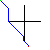
\includegraphics[width=40mm]{Run_0.png}
\caption{Small Cross Map. 50x50 pixel, with a start point of (0,0)}
\label{default}
\end{center}
\end{figure}

\begin{figure}[htbp]
\begin{center}
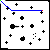
\includegraphics[width=40mm]{Run_6.png}
\caption{Small Area Of Regard, version 1. with a 50x50 pixel, start point of (0,0)}
\label{default}
\end{center}
\end{figure}

\begin{figure}[htbp]
\begin{center}
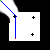
\includegraphics[width=40mm]{Run_9.png}
\caption{Small Area Of Regard, version 2. with a 50x50 pixel, start point of (0,0)}
\label{default}
\end{center}
\end{figure}


\begin{figure}[htbp]
\begin{center}
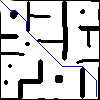
\includegraphics[width=60mm]{Run_1.png}
\caption{Medium  Map. 100x100 pixel, with a start point of (0,0)}
\label{default}
\end{center}
\end{figure}



\begin{figure}[htbp]
\begin{center}

\includegraphics[width=100mm]{Run_2.png}
\caption{Large Geometric Map. 1000x1000 pixel, with a start point of (0,0)}
\label{default}
\end{center}
\end{figure}

\begin{figure}[htbp]
\begin{center}
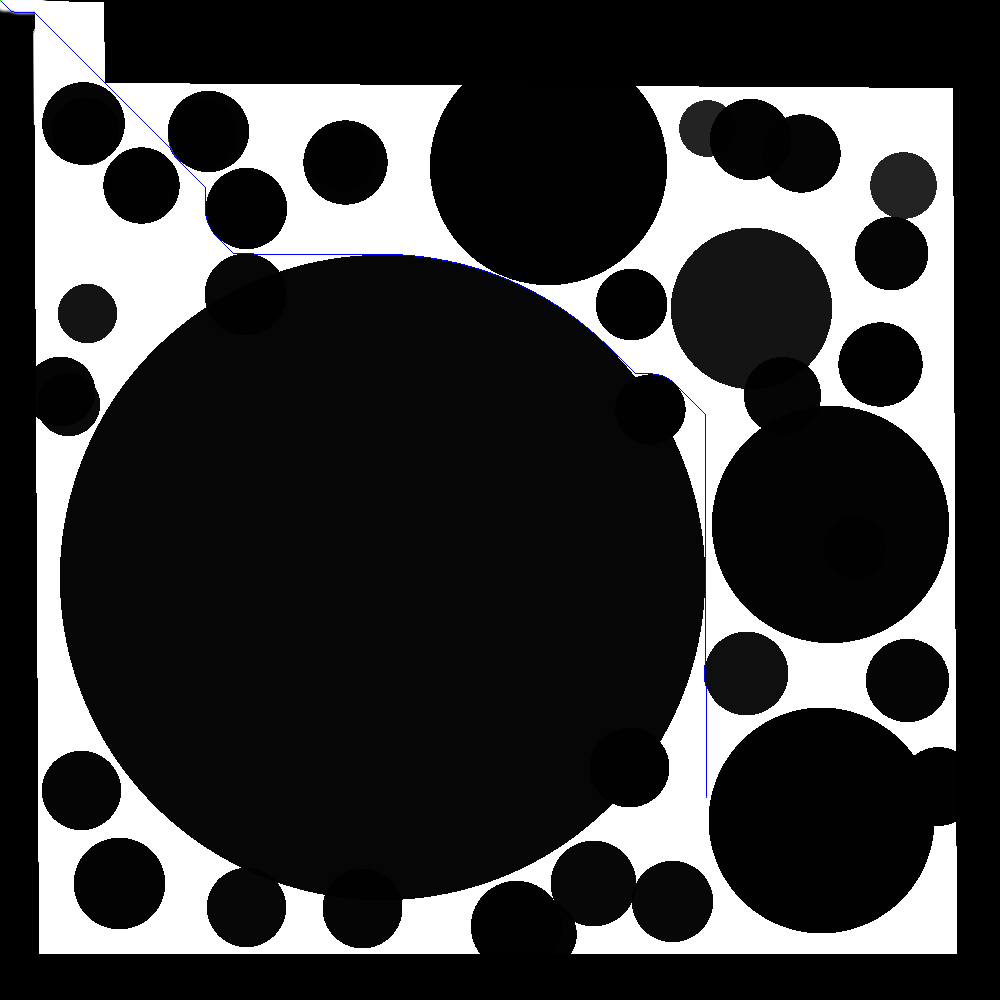
\includegraphics[width=100mm]{Run_3.png}
\caption{Large Area of Regard Map. 1000x1000 pixel, with a start point of (0,0)}
\label{default}
\end{center}
\end{figure}

\begin{figure}[htbp]
\begin{center}
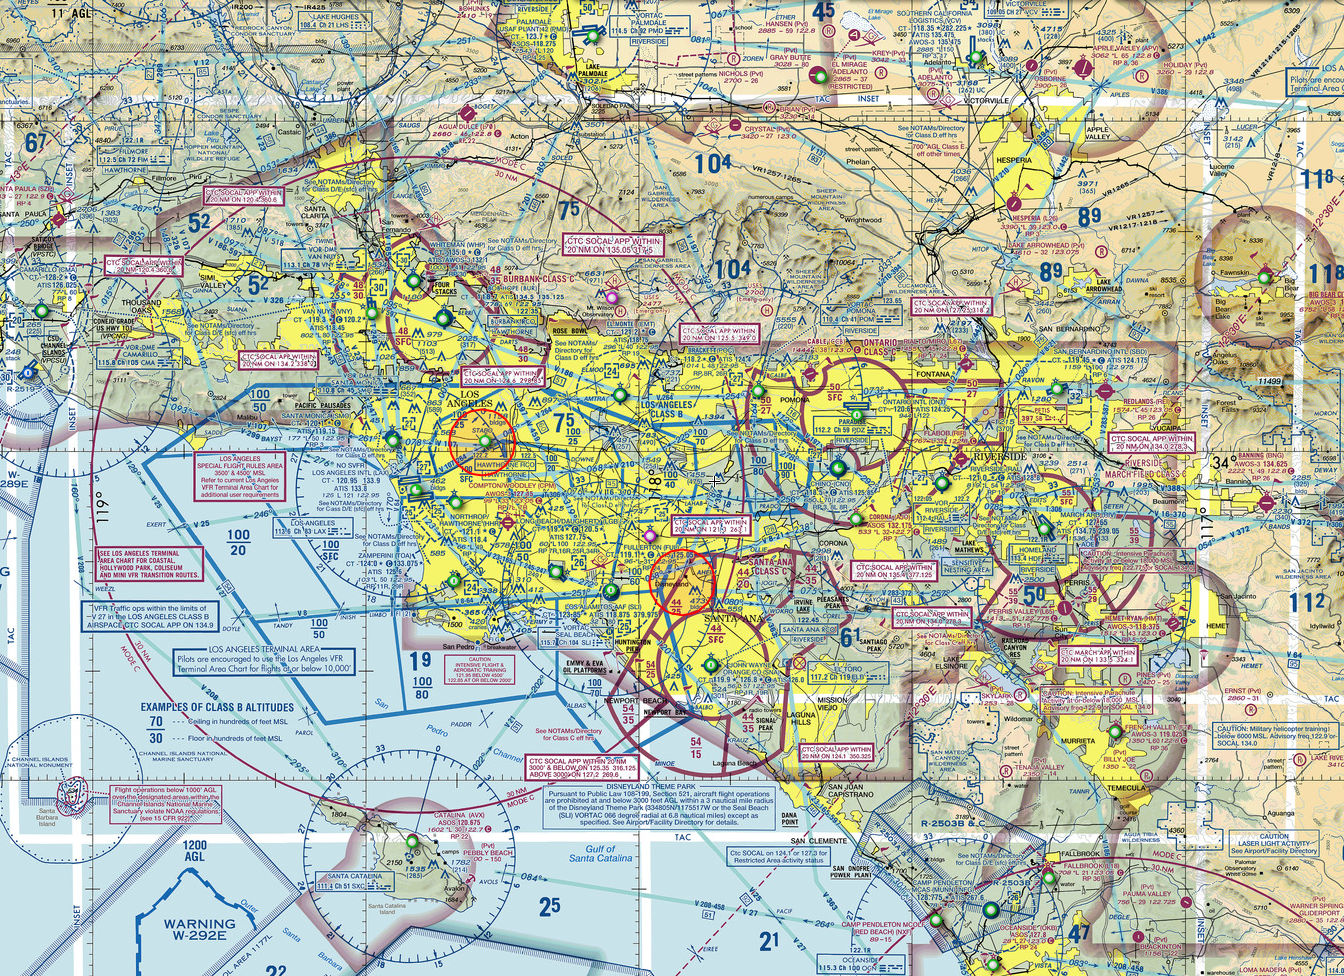
\includegraphics[width=130mm]{LAX.png}
\caption{Los Angeles Airspace}
\label{LAX}
\end{center}
\end{figure}


%%% End document
\end{document}